\usetikzlibrary{arrows.meta,calc,patterns,positioning}

\begin{frame}{memory v. disk}
\begin{tikzpicture}
\tikzset{
    mylabel/.style={font=\ttfamily},
    mybox/.style={draw,rectangle,minimum width=5cm,fill=white},
    myboxD/.style={draw,rectangle,minimum width=6cm,fill=white},
    myhigh/.style={draw,rectangle,line width=1mm, draw=blue!80!black,opacity=.3},
    nomem/.style={black!50,draw=black,fill=white},
}
\node[mybox,minimum height=1cm,pattern=north west lines,pattern color=black!20!white] (kernel) {Used by OS};
\node[above=.2cm of kernel] {(virtual) memory};
\node[mybox, minimum height=.5cm, below=1cm of kernel] (stack) {Stack};
\node[mybox, minimum height=.5cm, below=1cm of stack] (heap) {Heap / other dynamic};
\node[mybox, minimum height=.5cm, below=0mm of heap] (data) {Writable data};
\node[mybox, minimum height=.5cm, below=0mm of data] (sdata) {Code + Constants};
\coordinate (memBottom) at ($(sdata.south east) + (0mm, -2mm)$);
\begin{pgfonlayer}{bg}
\draw[pattern=north west lines, pattern color=black!40!white] (kernel.north west) rectangle (memBottom);
\end{pgfonlayer}

\node[myboxD,below right=4cm and 1cm of kernel,nomem] (diskHeader) {program header};
\node[myboxD,above=0cm of diskHeader] (textSeg) { {\tt .text} (code) };
\node[myboxD,above=0cm of textSeg] (rodataSeg) { {\tt .rodata} (read-only data) };
\node[myboxD,above=0cm of rodataSeg] (dataSeg) { {\tt .data} };
\node[myboxD,above=0cm of dataSeg,pattern=north west lines, pattern color=black!40] (bssSeg) { {\tt .bss} (zeroes; not stored) };
\node[above=.2cm of bssSeg] {program on disk};
\draw[very thick,-Latex] ([xshift=2mm]diskHeader.south east) -- ([xshift=2mm]bssSeg.north east) node[font=\small,midway,right,align=left] {higher \\ addresses \\ (and offsets)};


\foreach \f/\t in {textSeg/sdata,rodataSeg/sdata,dataSeg/data,bssSeg/data} {
    \draw[thick,-Latex,black] (\f.west) -- (\t.east);
}
\end{tikzpicture}

% FIXME: add animation: binary file format
\end{frame}

\begin{frame}{ELF (executable and linking format)}
\begin{itemize}
\item Linux {\small (and some others)} executable/object file format
\end{itemize}
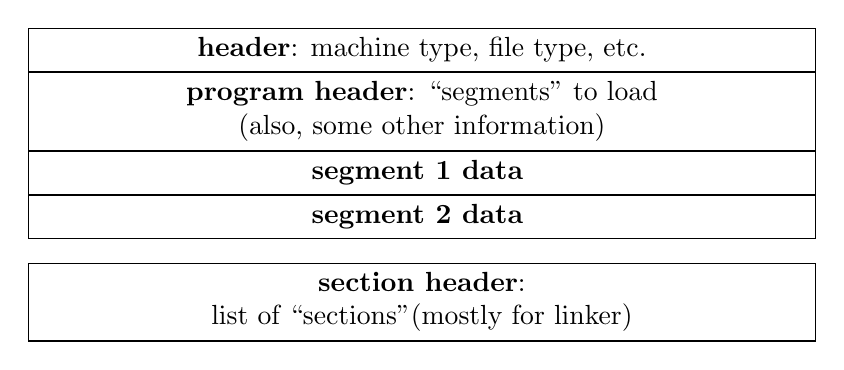
\begin{tikzpicture}
\tikzset{
    mybox/.style={draw,rectangle,minimum width=10cm,fill=white},
}
\node[mybox] (header) {
    \textbf{header}: machine type, file type, etc.
};
\node[mybox,below=0mm of header,align=center] (pHeader) {
    \textbf{program header}: ``\myemph{segments}'' to load \\
        (also, some other information)
};
\node[mybox,below=0mm of pHeader,align=center] (seg1) {
    \textbf{segment 1 data}
};
\node[mybox,below=0mm of seg1,align=center] (seg2) {
    \textbf{segment 2 data}
};
\node[mybox,below=3mm of seg2,align=center] (seg2) {
    \textbf{section header}:  \\ list of ``\myemph{sections}''(mostly for linker)
};
\end{tikzpicture}
\end{frame}

\begin{frame}{segments versus sections?}
\begin{itemize}
    \item note: ELF terminology; may not be true elsewhere!
    \item sections --- \myemph{object files} {\small (and usually executables)}, used by \myemph{linker}
        \begin{itemize}
        \item have information on intended purpose
        \item linkers combine these to create executables
        \item linkers might omit unneeded sections
        \end{itemize}
    \item segments --- executables, used to actually load program
        \begin{itemize}
        \item program loader is \myemph{dumb} --- doesn't know what segments are for
        \end{itemize}
\end{itemize}
\end{frame}

